\documentclass[UTF8]{ctexbeamer}	% Compile at least twice!
%\setbeamertemplate{navigation symbols}{}
\usetheme{Madrid}
% \setbeamertemplate{navigation symbols}{}
% \useinnertheme{rectangles}
% \useoutertheme{infolines}
% \useoutertheme[title,section,subsection=true]{smoothbars}
\useoutertheme{split}
\useinnertheme{rounded}
\setbeamertemplate{headline}{}
\usecolortheme{beaver}


% \usecolortheme{default}
% \usecolortheme{whale}
 
% -------------------
% Packages
% -------------------
\usepackage{
    amsmath,			% Math Environments
    amssymb,			% Extended Symbols
    enumerate,		    % Enumerate Environments
    graphicx,			% Include Images
    lastpage,			% Reference Lastpage
    multicol,			% Use Multi-columns
    multirow,			% Use Multi-rows
    pifont,			    % For Checkmarks
    stmaryrd,            % For brackets
    listings,
    subfigure,
}
\usepackage[english]{babel}
\usepackage{graphicx}
\usepackage{animate}
\usepackage{xeCJK}
\usepackage{fontspec} 
% \setmainfont{KaiTi_GB2312}
% \setCJKmainfont{KaiTi_GB2312}
% \setmainfont{Source Han Sans CN Medium} 
% \setCJKmainfont{Source Han Sans CN Medium}

\setmainfont{Source Code Pro}
% \setmainfont{Sarasa Mono CL}
\setCJKmainfont{Sarasa Mono CL}

% \newfontfamily\os{Open Sans}
% \newfontfamily\oscl{Open Sans Condensed}
% \newfontfamily\tnr{Times New Roman}
% \newfontfamily\tnrc{Times New Roman Cyr}
% \newfontfamily\tim{Times}
% \newfontfamily\roc{Rockwell}
% \usepackage{CJK}
% \lstset{language=C++}
% \lstset{extendedchars=false}
% \lstset{breaklines}


% -------------------
% Colors
% -------------------
% \definecolor{UniOrange}{RGB}{212,69,0}
% \definecolor{UniGray}{RGB}{62,61,60}
% \definecolor{UniRed}{HTML}{B31B1B}
% \definecolor{UniGray}{HTML}{222222}
% \setbeamercolor{title}{fg=UniGray}
% \setbeamercolor{frametitle}{fg=UniOrange}
% \setbeamercolor{structure}{fg=UniOrange}
% \setbeamercolor{section in head/foot}{bg=UniGray}
% \setbeamercolor{author in head/foot}{bg=UniGray}
% \setbeamercolor{date in head/foot}{fg=UniGray}
% \setbeamercolor{structure}{fg=UniOrange}
% \setbeamercolor{local structure}{fg=black}
% \beamersetuncovermixins{\opaqueness<1>{0}}{\opaqueness<2->{15}}


% -------------------
% Fonts & Layout
% -------------------
% \usepackage{palatino}
\usefonttheme{serif}
% \setbeamerfont{title like}{shape=\scshape}
% \setbeamerfont{frametitle}{shape=\scshape}
% \setbeamertemplate{itemize items}[circle]
% \setbeamertemplate{enumerate items}[default]


% -------------------
% Commands
% -------------------

% Special Characters
% \newcommand{\N}{\mathbb{N}}
% \newcommand{\Z}{\mathbb{Z}}
% \newcommand{\Q}{\mathbb{Q}}
% \newcommand{\R}{\mathbb{R}}
%\newcommand{\C}{\mathbb{C}}

% Math Operators
% \DeclareMathOperator{\im}{im}
% \DeclareMathOperator{\Span}{span}

% Special Commands
% \newcommand{\pf}{\noindent\emph{Proof. }}
% \newcommand{\ds}{\displaystyle}
% \newcommand{\defeq}{\stackrel{\text{def}}{=}}
% \newcommand{\ov}[1]{\overline{#1}}
% \newcommand{\ma}[1]{\stackrel{#1}{\longrightarrow}}
% \newcommand{\twomatrix}[4]{\begin{pmatrix} #1 & #2 \ #3 & #4 \end{pmatrix}}


% -------------------
% Tikz & PGF
% -------------------
\usepackage{tikz}
\usepackage{tikz-cd}
\usetikzlibrary{
    calc,
    decorations.pathmorphing,
    matrix,arrows,
    positioning,
    shapes.geometric
}
\usepackage{pgfplots}
\pgfplotsset{compat=newest}
\usepackage{wrapfig}
\usepackage{cite}


% -------------------
% Theorem Environments
% -------------------
\usepackage{amsthm}
\theoremstyle{plain}
\newtheorem{sit}{Situation}[section]
\newtheorem{prop}{Proposition}[section]
\newtheorem{rtm}{Theorem}[section]
\newtheorem{cor}{Corollary}[section]
\theoremstyle{definition}
\newtheorem{das}{Data structure}[section]
\newtheorem{nex}{Non-Example}[section]
\newtheorem{cla}{class}[section]
\newtheorem{emt}{}[section]
\newtheorem{defn}{Definition}[section]
\theoremstyle{remark}
\newtheorem{rem}{Remark}[section] 
\numberwithin{equation}{section}

\newcommand\caesura{$\mkern -8.5mu\raise -.2ex\hbox{\rotatebox[]{180}{\`}}\ $}
\setbeamertemplate{caption}[numbered]
% -------------------
% Title Page
% -------------------
\title{\textcolor{red}{三维殷集程序进展}}
%\subtitle{\textcolor{white}{Mathematics Conference for the Mysterious and dMagical}}  
\author{谭焱, 邱云昊 
% \newline \newline
%  \small{硕士导师: 王何宇\, \\
%  申请博士导师: 张庆海}
 }

% \institute{\small{现硕士导师: 王何宇 、张庆海 \newline 拟转博士指导教师: 张庆海} \newline   \newline 浙江大学数学科学学院}
\date{\today} 


% -------------------
% Content
% -------------------
\begin{document}
% \begin{CJK}{GBK}{kai}

% Title Page
\begin{frame}
    \titlepage
\end{frame}


\begin{frame}
    \frametitle{提纲}
    \tableofcontents
\end{frame}

\section{程序背景}

% \subsection{\textcolor{red}{}}
\begin{frame}
    \frametitle{殷集研究背景}
    \begin{itemize}
        \item 多相流中的几何和拓扑问题是求解动边界偏微分方程的核心问题.
        \item 现有方法对界面的几何和拓扑问题进行回避,导致了:
              \begin{enumerate}
                  \item 对等距变换的流场不能保证几何性质.
                  \item 对同胚映射的流场不能保证拓扑性质.
                  \item 精度最高为二阶精度.
                  \item 很难对拓扑变化进行严格的处理.
              \end{enumerate}
        \item 我们的核心思想是用\textcolor{red}{几何和拓扑的手段
                  研究几何和拓扑的问题},其中首要工作在于殷集对流相建模.
    \end{itemize}
    \begin{columns}
        \column{0.4\linewidth}<1->
        \centering
        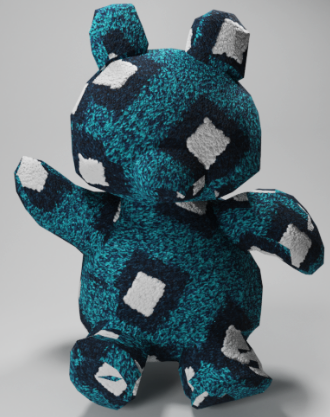
\includegraphics[width = .6\textwidth]{fig/s18.png}
        \column{0.6\linewidth}<1->
        \centering
        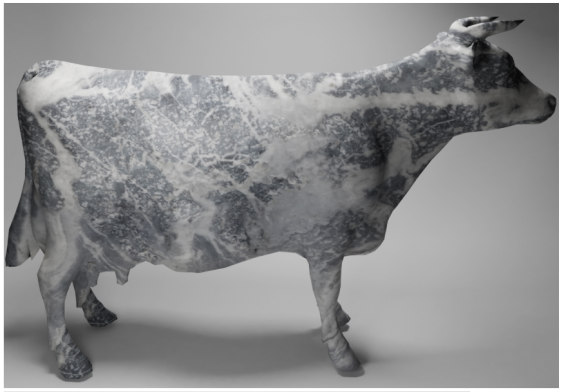
\includegraphics[width = .7\textwidth]{fig/s19.png}
    \end{columns}
\end{frame}


\begin{frame}
    \frametitle{二维殷集}
    \begin{itemize}
        \item \textcolor{red}{殷集}:空间中边界有界的正则半解析开集.所有殷集构
              成的集合被称为殷空间,记为 $\mathbb{Y}$.
        \item 二维空间中,任一个殷集可以唯一表示为
              \[\mathcal{Y} = \cup_j^{\bot \bot}\cap_i \text{int}(\gamma_{j, i} ),\]
              约当曲线 $\gamma_{j, i}$是$\mathcal{Y}$内第$j$个连通分量
              的第$i$条边界.
        \item 实现了殷集上的布尔代数.
    \end{itemize}
    \begin{figure}[!htb]
        \centering
        \subfigure{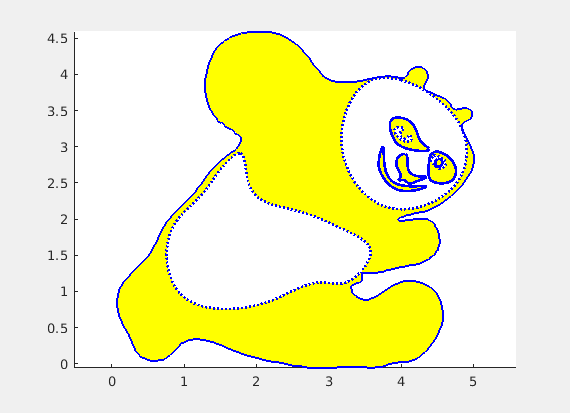
\includegraphics[width=0.3\textwidth]{fig/p.png}}
        \subfigure{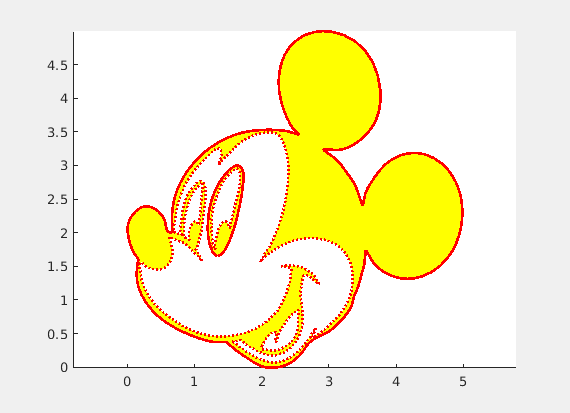
\includegraphics[width=0.3\textwidth]{fig/m.png}}
        \subfigure{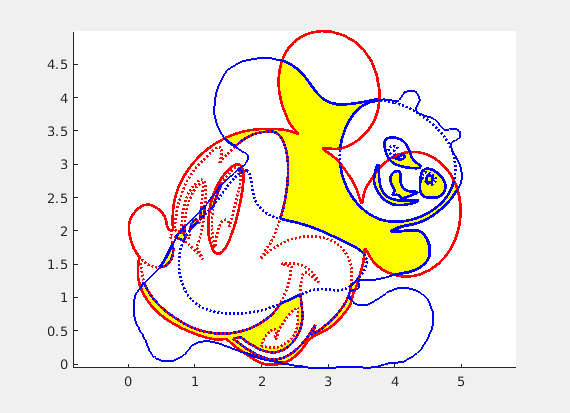
\includegraphics[width=0.3\textwidth]{fig/pm.png}}
        \caption{二维殷集的交}
        %   \vspace{0.2in}
    \end{figure}
\end{frame}

\begin{frame}
    \frametitle{黏合紧曲面}
    \begin{itemize}
        \item
              \textcolor{red}{二流形的分类定理} \newline
              有向的二维紧流形同胚于球面或轮胎面或轮胎面的连通和.
              \begin{figure}[!htb]
                \centering
                \subfigure{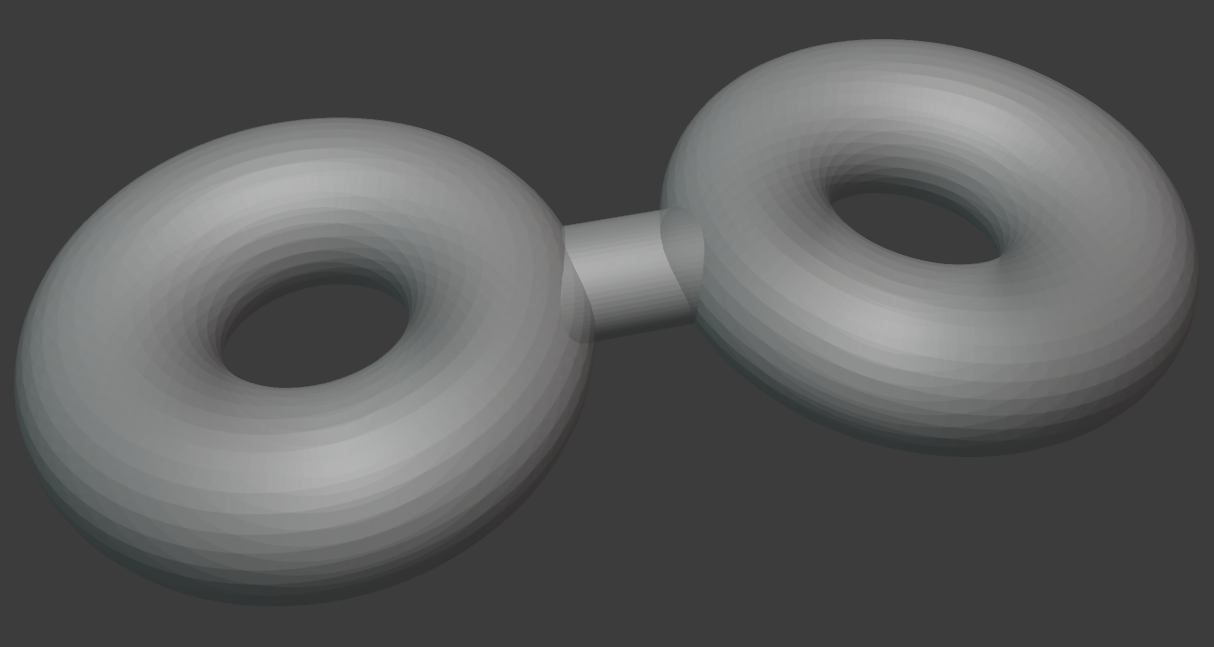
\includegraphics[width=0.4\textwidth]{fig/connectsum.png}} \qquad
                \subfigure{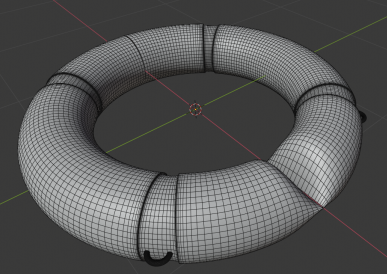
\includegraphics[width=0.3\textwidth]{fig/past.png}}
            \end{figure}


        \item 黏合紧曲面是一个二维连通紧流形或这种流形的商空间, 其商映射
              将紧流形与一维 CW 复形同胚的子集粘在一起; 将这个一维子集删除后
              该黏合紧曲面仍然是连通的.
    \end{itemize}
\end{frame}

\begin{frame}
    \frametitle{三维殷集的唯一表示}
    \begin{itemize}
        \item 任一个殷集$\mathcal{Y} \in \mathbb{Y}$可以唯一表示为
              \[\mathcal{Y} = \cup_j^{\bot \bot} \cap_i \text{int}(\Gamma_{j, i}),\]
              黏合紧曲面$\Gamma_{j, i}$是$\mathcal{Y}$的第$j$个连通分量的第$i$个边界.
        \item 连通分量个数等于正向黏合紧曲面的个数(有界殷集)或正向黏合紧曲面个数+1(无界殷集).

        \item 洞的个数等于负向黏合紧曲面的个数.
    \end{itemize}
    \begin{columns}
        \column{0.35\linewidth}<1->
        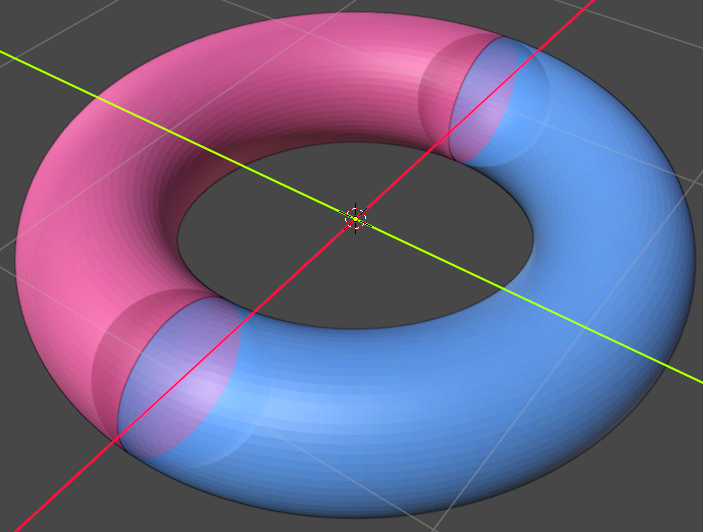
\includegraphics[width = \textwidth]{fig/ys1.png}
        \column{0.35\linewidth}<1->
        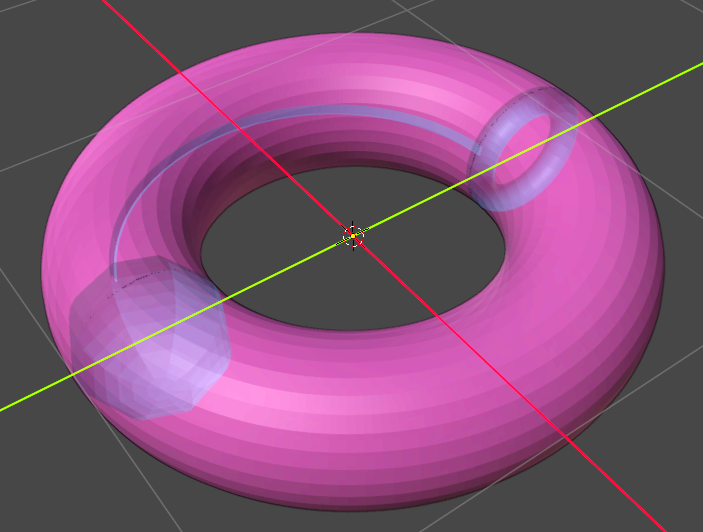
\includegraphics[width = \textwidth]{fig/ys5.png}
    \end{columns}
\end{frame}

\section{程序进展}
\subsection{程序架构}
\begin{frame}
    \frametitle{布尔代数程序的实现方式}
    \begin{itemize}
        \item 实现步骤
    \begin{enumerate}
        \item 计算一个殷集边界上的自交线或两个殷集之间的交线.
        \item 黏合紧曲面沿交线剪开得到若干曲面片.
        \item 根据交并补的需要删除曲面片或改变曲面片方向.
        \item 将曲面片重新粘合成黏合紧曲面集合.
        \item 黏合紧曲面集合唯一表示一个三维殷集作为布尔运算结果.
    \end{enumerate}

        \item 代码模块
        \begin{enumerate}
            \item class TriangleIntersection. 找到交线.
            \item class Triangulation. 沿交线重新三角化.
            \item class Prepaste. 沿交线剪开得到曲面片.
            \item class RemoveOverlap. 恰当的保留曲面片.
            \item class Locate. 恰当的保留曲面片.
            \item class Paste. 生成黏合紧曲面.
            \item YinSet(). 构造殷集.
        \end{enumerate}
    \end{itemize}
\end{frame}

\begin{frame}
    \frametitle{时间瓶颈分析}
    \begin{itemize}
        \item 求交运算在同一图形的不同加密次数的模型上计算时间.
        \begin{table}[]
            \resizebox{0.9\textwidth}{!}{%
            \begin{tabular}{|l|l|l|l|l|l|l|}
            \hline
            三角形/个 & 求交/秒 & Ratio & 三角化/秒 & Ratio & 总时间 & Ratio \\ \hline
$2.11 \times 10^3$ & $5.52 \times 10^{-1}$ &      & $1.63 \times 10^{-1}$ &      & $7.63 \times 10^{-1}$ &
\\ \hline
$3.46 \times 10^4$ & $1.04 \times 10^{2}$  & 1.87 & $2.33 \times 10^{0}$  & 0.95 & $1.07 \times 10^{2}$  & 1.76
\\ \hline
$1.14 \times 10^5$ & $1.26 \times 10^{3}$  & 2.09 & $7.66 \times 10^{0}$  & 0.99 & $1.27 \times 10^{3}$  & 2.07
\\ \hline
$3.59 \times 10^5$ & $1.28 \times 10^{4}$  & 2.02 & $2.42 \times 10^{1}$  & 1.00 & $1.29 \times 10^{4}$  & 2.02
\\ \hline
$5.39 \times 10^5$ & $2.89 \times 10^{4}$  & 2.00 & $3.59 \times 10^{1}$  & 0.97 & $2.90 \times 10^{4}$  & 1.99
\\ \hline
            \end{tabular}
            }
            \end{table}

            \item 三角形求交和三角化占用求交程序大部分时间.
            \item 计算时间过长,瓶颈在三角形求交,需求
            时间复杂度更低的求交算法.
            
            \item 三角化的时间复杂度达到理论最优的$O(n)$.
    \end{itemize}
\end{frame}

\subsection{计算交线的优化}
\begin{frame}
    \frametitle{使用空间划分降低求交计算时间度}
    \begin{itemize}
        \item 三角形相交局部发生, 将三角形划分到不同的局部降低计算量.
        \item 建立空间八叉树结构, 通过剪枝实现自适应细化.
        \item 假设三角形分布均匀可证计算时间复杂度为$O(nlogn)$.
        \begin{center}
            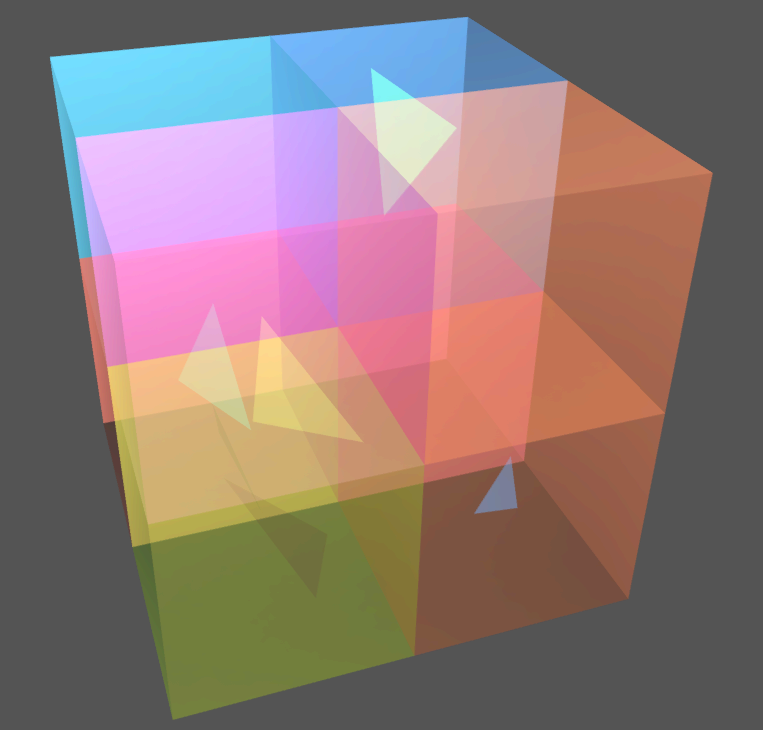
\includegraphics[width = 0.3\textwidth]{fig/treeem.png}
        \end{center} 
        \begin{table}[]
            \resizebox{0.6\textwidth}{!}{%
            \begin{tabular}{|l|l|l|l|l|}
            \hline
            三角形/个 & 两两求交/秒 & Ratio & 空间划分/秒 & Ratio \\ \hline
$2.11 \times 10^3$ & $5.52 \times 10^{-1}$ &      & $4.26 \times 10^{-1}$ & 
\\ \hline
$3.46 \times 10^4$ & $1.04 \times 10^{2}$  & 1.87 & $5.14 \times 10^{0}$  & 0.89 
\\ \hline
$1.14 \times 10^5$ & $1.26 \times 10^{3}$  & 2.09 & $1.36 \times 10^{1}$  & 0.82 
\\ \hline
$3.59 \times 10^5$ & $1.28 \times 10^{4}$  & 2.02 & $3.44 \times 10^{1}$  & 0.80 
\\ \hline
$5.39 \times 10^5$ & $2.89 \times 10^{4}$  & 2.00 & $4.85 \times 10^{1}$  & 0.84 
\\ \hline
            \end{tabular}
            }
            \end{table}
    \end{itemize}
\end{frame}

\begin{frame}
    \frametitle{针对殷集与网格求交优化}
    \begin{itemize}
    \item 有限体积法基于网格的控制体,求解需大量控制体和殷集求交,使用前面的方法耗时过长,因此设计了一种加速的算法.
    \item 将殷集的每个三角形与所有与之相交的网格面求交得到若干交线.
      \item 将每条交线沿着网格面中的网格进行剪切得到若干交线段.
      \item 殷集与网格结合交线段完成三角化.
        % \item 这种求交的优点是不存在重复或不必要的求交.
        \vspace{0.2in}
         \begin{columns}
        \column{0.4\linewidth}<1->
        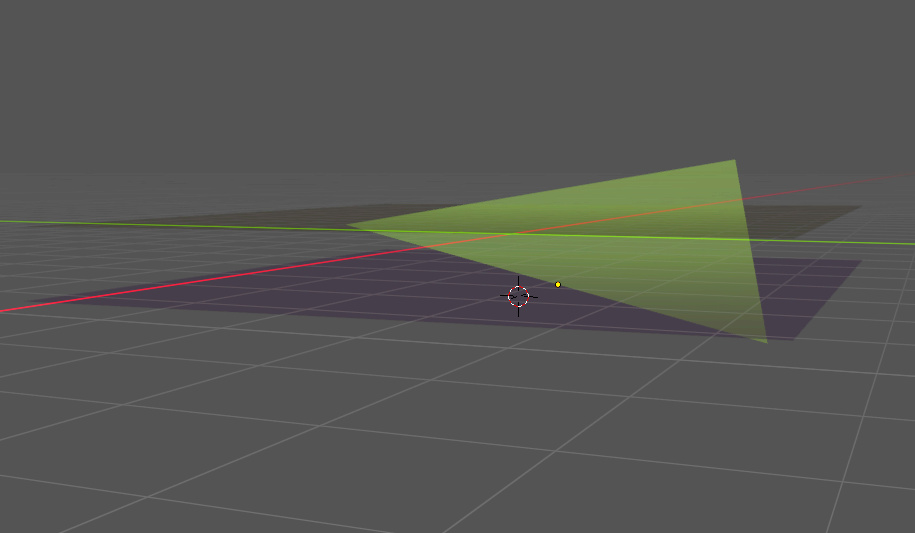
\includegraphics[width = \textwidth]{fig/swem.png}
        \column{0.4\linewidth}<1->
        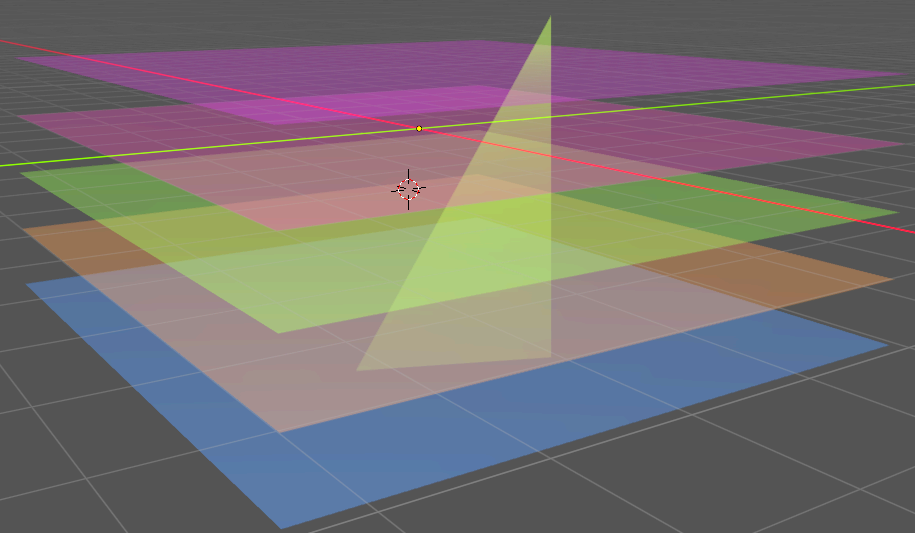
\includegraphics[width = \textwidth]{fig/sw2em.png}
    \end{columns}
    \end{itemize}
\end{frame}


\begin{frame}
    \frametitle{优化效果分析}
    \begin{itemize}
        \item 不妨假设三角形与至多常数$N$个网格面相交.
        \item 计算复杂度从$O(n_1  n_2)$降为$O(n_2)$.
        % \item 只需替换TriangleIntersection模块.
        \item 空间划分三角形求交与三角化计算时间接近,优化效果有待验证.
        \vspace{0.2in}
        \begin{table}[]
            \resizebox{0.7\textwidth}{!}{%
            \begin{tabular}{|l|l|l|l|l|}
            \hline
            三角形/个 & 空间划分/秒 & 比例 & 三角化/秒 & 比例   \\ \hline
$2.11 \times 10^3$ & $4.26 \times 10^{-1}$ & 0.72   & $1.63 \times 10^{-1}$ & 0.28    
\\ \hline
$3.46 \times 10^4$ & $5.14 \times 10^{0}$  & 0.69   & $2.33 \times 10^{0}$  & 0.31 
\\ \hline
$1.14 \times 10^5$ & $1.36 \times 10^{1}$  & 0.64   & $7.66 \times 10^{0}$  & 0.36 
\\ \hline
$3.59 \times 10^5$ & $3.44 \times 10^{1}$  & 0.59   & $2.42 \times 10^{1}$  & 0.41  
\\ \hline
$5.39 \times 10^5$ & $4.85 \times 10^{1}$  & 0.57   & $3.59 \times 10^{1}$  & 0.43 
\\ \hline
            \end{tabular}
            }
            \end{table}
%             & $1.63 \times 10^{-1}$ &      & $7.63 \times 10^{-1}$
% & $2.33 \times 10^{0}$  & 0.95 & $1.07 \times 10^{2}$ 
% & $7.66 \times 10^{0}$  & 0.99 & $1.27 \times 10^{3}$ 
% & $2.42 \times 10^{1}$  & 1.00 & $1.29 \times 10^{4}$ 
% & $3.59 \times 10^{1}$  & 0.97 & $2.90 \times 10^{4}$ 
    \end{itemize}
\end{frame}

\subsection{粘合模块的修改}
\begin{frame}
    \frametitle{原Paste方法的问题}
    \begin{itemize}
        \item 原Paste方法采用分类讨论证明粘合的正确性.
        % \item 原Past方法只证明了能将殷集正确黏合.
        % \item 没有检测到一些疑似殷集的非殷集输入.
        \vspace{0.2in}
        \begin{columns}
       \column{0.35\linewidth}<1->
       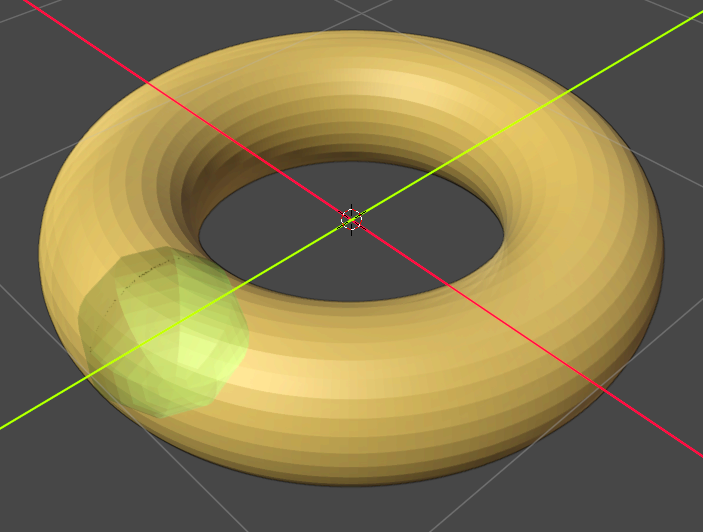
\includegraphics[width = \textwidth]{fig/ys4.png}
       \column{0.35\linewidth}<1->
       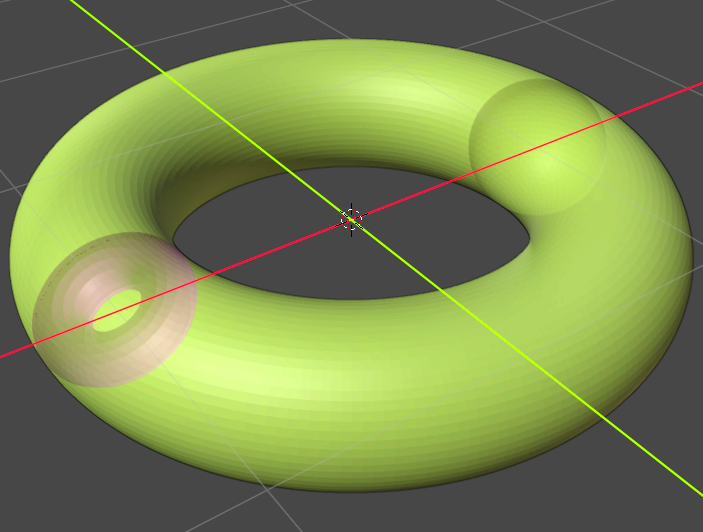
\includegraphics[width = \textwidth]{fig/ys2.png}
   \end{columns}
   \vspace{0.1in}
   \begin{columns}
    \column{0.35\linewidth}<1->
    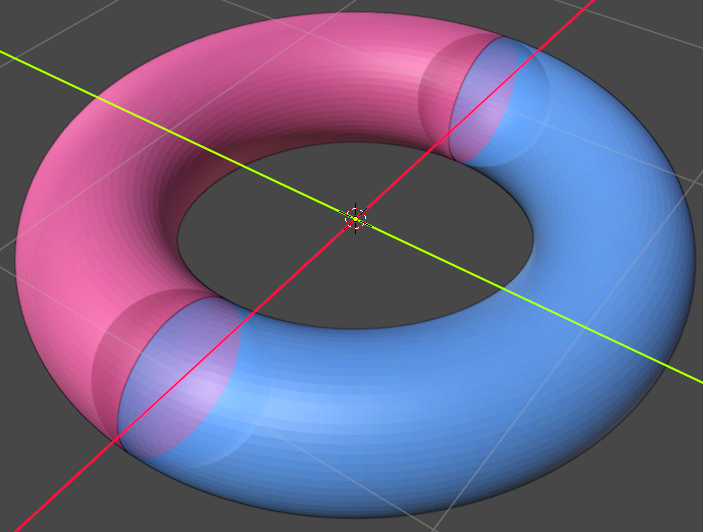
\includegraphics[width = \textwidth]{fig/ys1.png}
    \column{0.35\linewidth}<1->
    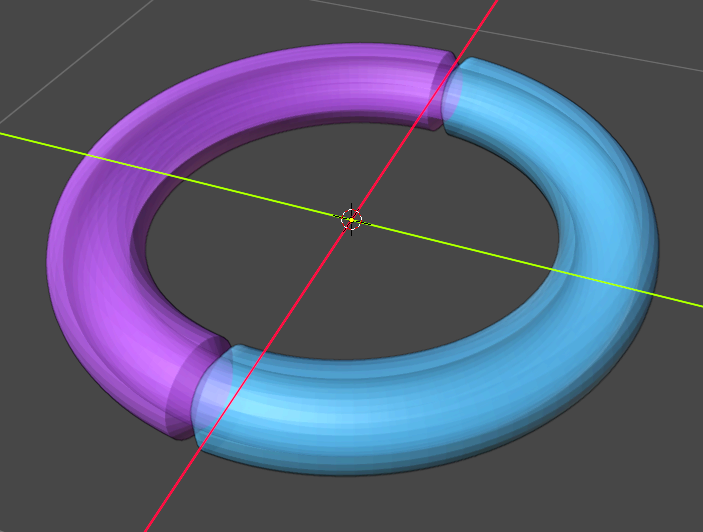
\includegraphics[width = \textwidth]{fig/ys3.png}
\end{columns}
    \end{itemize}
\end{frame}

\begin{frame}
    \frametitle{黏合紧曲面的性质}
    \begin{center}
        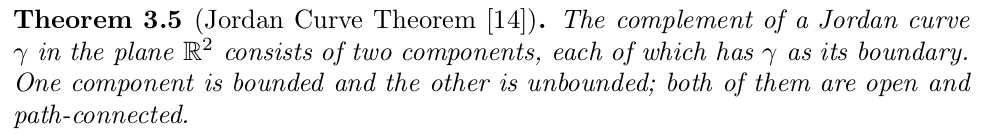
\includegraphics[width = 0.9\textwidth]{fig/jordancurve.png}
    \end{center}
    \vspace{-0.2in}
        \begin{itemize}
            \item 黏合紧曲面同样拥有类似性质.
            \item 黏合紧曲面是一个二维连通紧流形或这种流形的商空间, 其商映射
            将紧流形与一维 CW 复形同胚的子集粘在一起; 将这个一维子集删除后
            该黏合紧曲面仍然是连通的.
            % \vspace{-0.1in}
            \begin{center}
                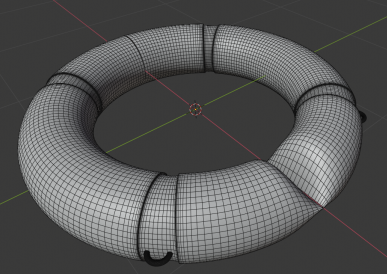
\includegraphics[width = 0.4\textwidth]{fig/past.png}
            \end{center}
        \end{itemize}
\end{frame}

\begin{frame}
    \frametitle{生成黏合紧曲面的方法}
    \begin{itemize}
      \item 好配对黏合: 始终沿着一个连通分量黏合.
        \item 好配对黏合不一定是黏合紧曲面.
        \item 对于好配对黏合得到的连通分量的边界,沿自交线剪开反向并重新进行好配对黏合(这时一定得到黏合紧曲面),将黏合得到的若干反向的黏合紧曲面再反向可以得到正确定向的黏合紧曲面.
        % \item 该方法检测到Rabbit不为殷集.
    \end{itemize}
    \vspace{0.1in}
     \begin{columns}
        \column{0.35\linewidth}<1->
        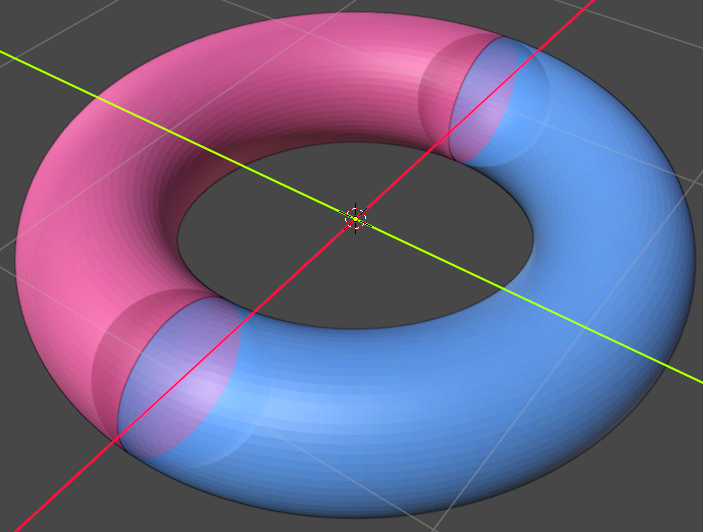
\includegraphics[width = \textwidth]{fig/ys1.png}
        \column{0.35\linewidth}<1->
        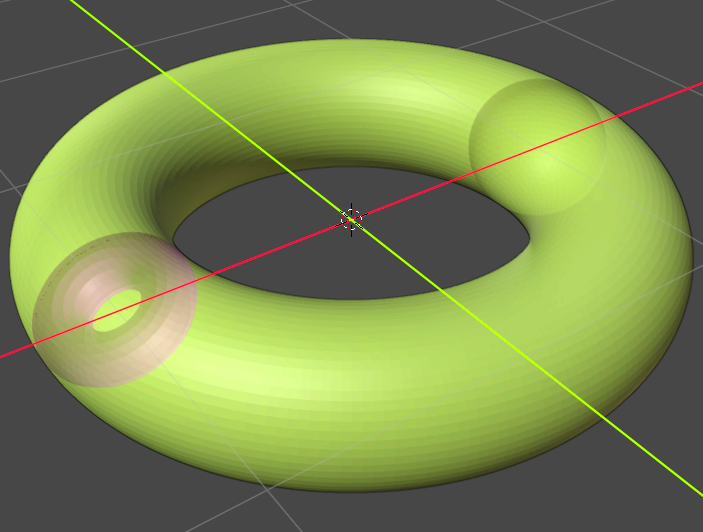
\includegraphics[width = \textwidth]{fig/ys2.png}
    \end{columns}
\end{frame}

\section{后续工作}
\begin{frame}
    \frametitle{缺乏几何结构复杂的模型}
    \begin{columns}
        \column{0.3\linewidth}<1->
        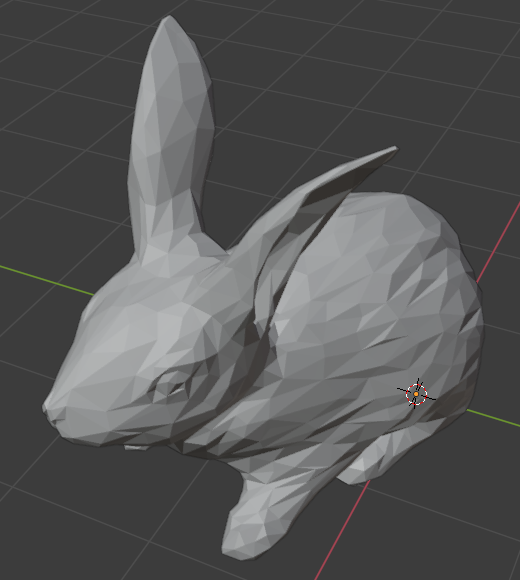
\includegraphics[width = \textwidth]{fig/wrong1.png}
        \column{0.3\linewidth}<1->
        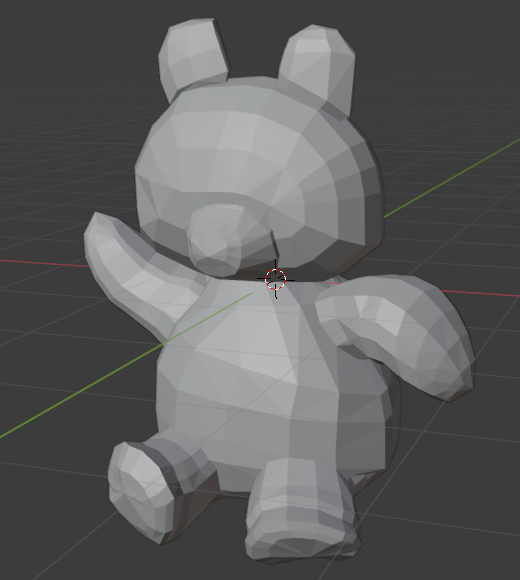
\includegraphics[width = \textwidth]{fig/wrong2.png}
        \column{0.32\linewidth}<1->
        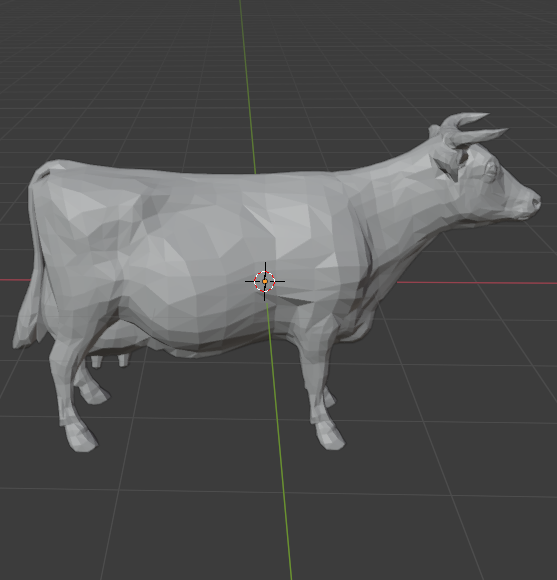
\includegraphics[width = \textwidth]{fig/wrong3.png}
    \end{columns}
    \begin{columns}
        \column{0.65\linewidth}<1->
    \begin{enumerate}
        \item Rabbit与Teddy内部洞边界的方向朝外.
        \item cow尾部有不可定向的曲面片.
        \item 缺乏几何结构复杂的殷集测试模型.
    \end{enumerate}
    \column{0.3\linewidth}<1->
    \begin{figure}[htbp]
        \flushright
        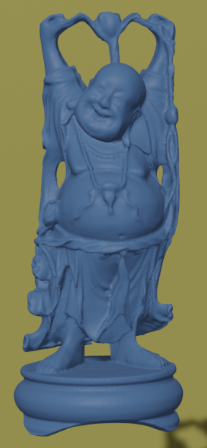
\includegraphics[width = 0.4
        \textwidth]{fig/wrong4.png}
    \end{figure}
    \end{columns}

\end{frame}

\begin{frame}
    \frametitle{通用三维测试模型的问题}
    \begin{columns}
        \column{0.4\linewidth}<1->
        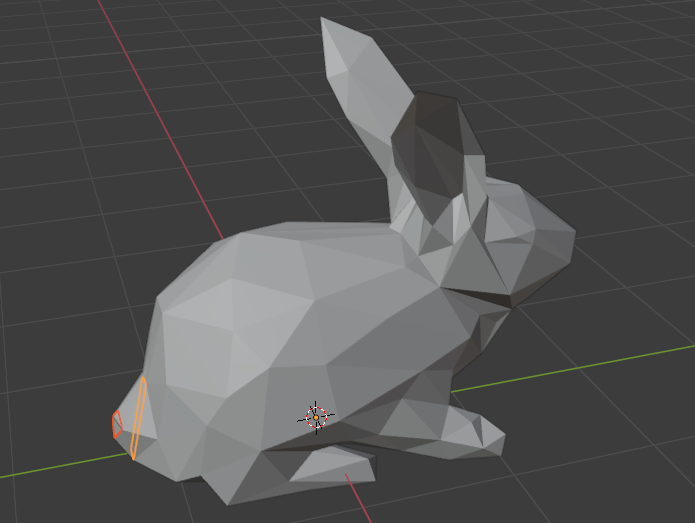
\includegraphics[width = \textwidth]{fig/rabbit1.png}
        \column{0.4\linewidth}<1->
        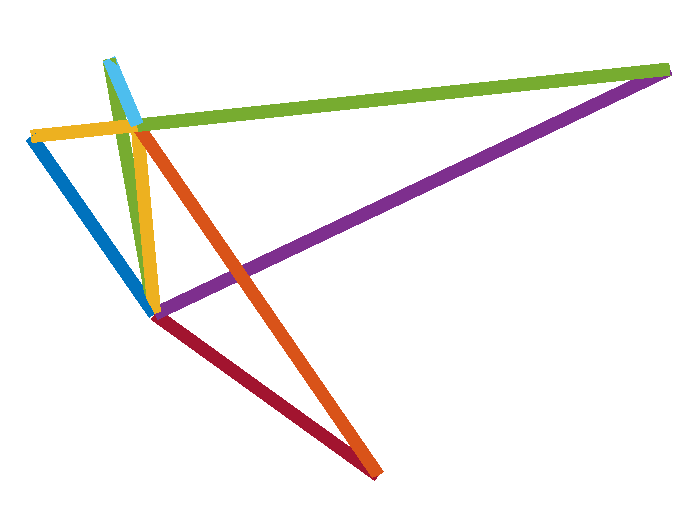
\includegraphics[width = \textwidth]{fig/rabbit2.png}
    \end{columns}
    \begin{columns}
        \column{0.3\linewidth}<1->
        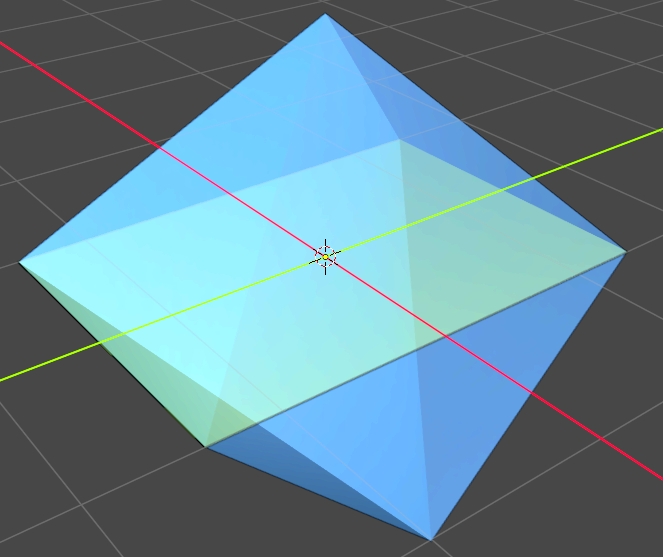
\includegraphics[width = \textwidth]{fig/wrong5em.png}
        \column{0.3\linewidth}<1->
        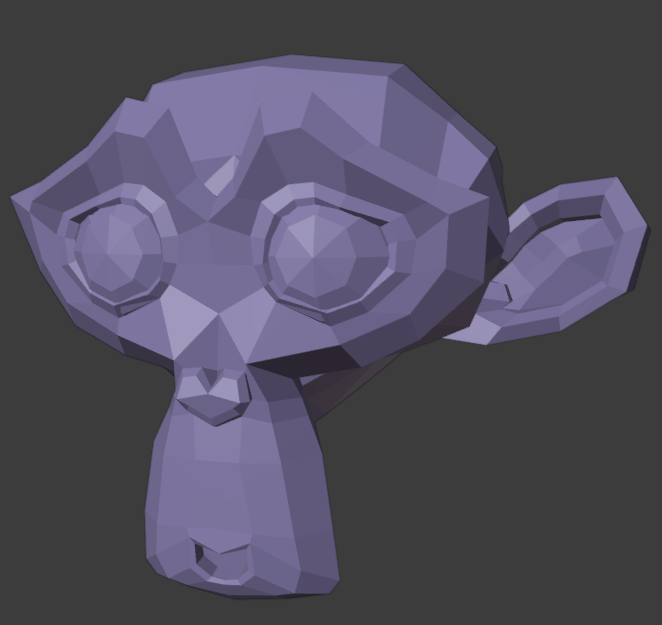
\includegraphics[width = \textwidth]{fig/wrong6.png}
        \column{0.23\linewidth}<1->
        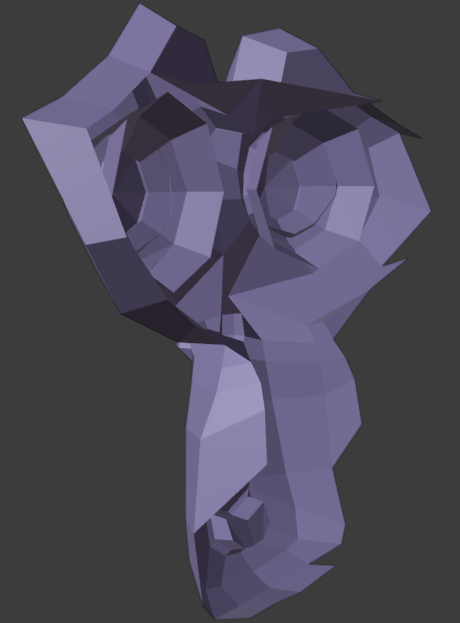
\includegraphics[width = \textwidth]{fig/wrong7.png}
        
    \end{columns}

\end{frame}

\begin{frame}
    \frametitle{后续工作方向}
    \begin{itemize}
        \item 增加测试样例.
        \begin{enumerate}
        \item 熟悉已完成的三维殷集表面建模程序.
        \item 截取简单殷集模型在复杂流场运行一段时间后的殷集.
        \item 使用blender构建拓扑结构复杂的模型.
        \item 验证程序的正确性.
    \end{enumerate}
    
    \item 分析优化计算求交.
    \begin{enumerate}
        \item 分析布尔运算程序速度是否为瓶颈.
        \item 检索更优的三角形求交和三角化算法.
    \end{enumerate}

    \item 重构现有程序.
    \end{itemize}
\end{frame}


\section*{}
\begin{frame}
    \centering\huge
    \textcolor{red}{请老师同学批评指正!}
\end{frame}
\end{document}